% Created by tikzDevice version 0.12.6 on 2024-03-17 19:30:52
% !TEX encoding = UTF-8 Unicode
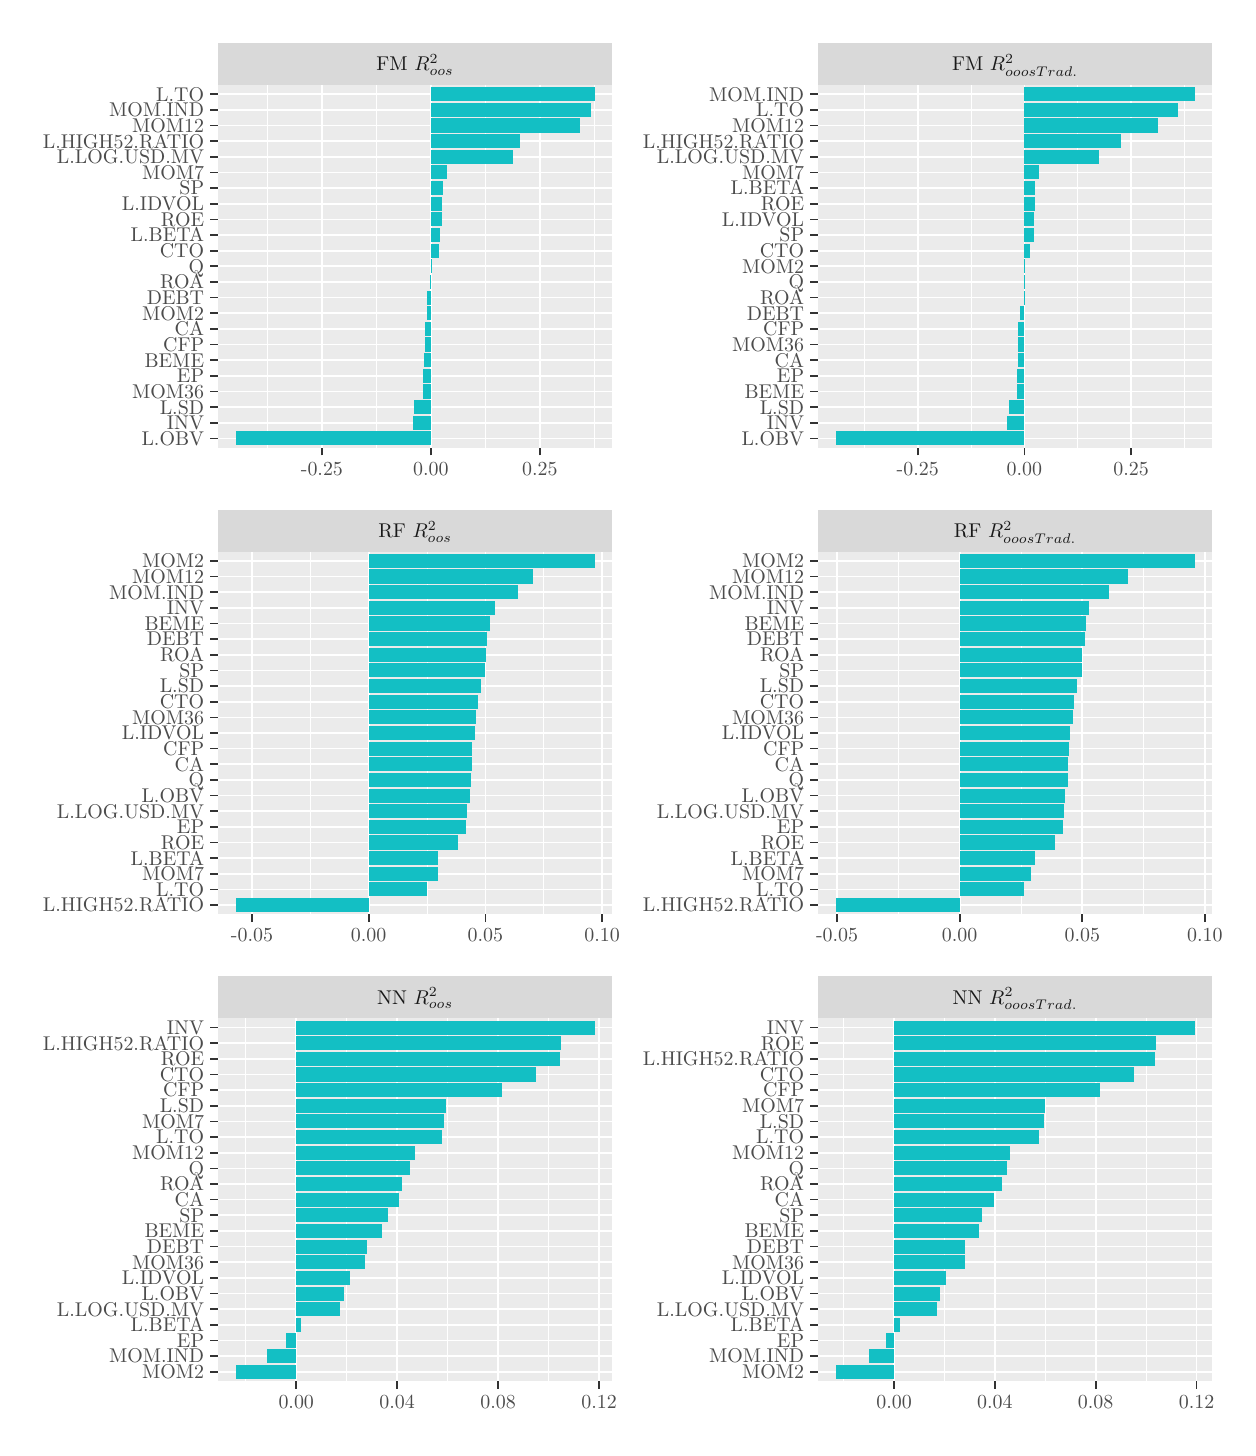
\begin{tikzpicture}[x=1pt,y=1pt]
\definecolor{fillColor}{RGB}{255,255,255}
\path[use as bounding box,fill=fillColor,fill opacity=0.00] (0,0) rectangle (433.62,505.89);
\begin{scope}
\path[clip] (  0.00,337.26) rectangle (216.81,505.89);
\definecolor{drawColor}{RGB}{255,255,255}
\definecolor{fillColor}{RGB}{255,255,255}

\path[draw=drawColor,line width= 0.6pt,line join=round,line cap=round,fill=fillColor] (  0.00,337.26) rectangle (216.81,505.89);
\end{scope}
\begin{scope}
\path[clip] ( 68.69,354.07) rectangle (211.31,485.23);
\definecolor{fillColor}{gray}{0.92}

\path[fill=fillColor] ( 68.69,354.07) rectangle (211.31,485.23);
\definecolor{drawColor}{RGB}{255,255,255}

\path[draw=drawColor,line width= 0.3pt,line join=round] ( 86.63,354.07) --
	( 86.63,485.23);

\path[draw=drawColor,line width= 0.3pt,line join=round] (126.01,354.07) --
	(126.01,485.23);

\path[draw=drawColor,line width= 0.3pt,line join=round] (165.39,354.07) --
	(165.39,485.23);

\path[draw=drawColor,line width= 0.3pt,line join=round] (204.77,354.07) --
	(204.77,485.23);

\path[draw=drawColor,line width= 0.6pt,line join=round] ( 68.69,357.46) --
	(211.31,357.46);

\path[draw=drawColor,line width= 0.6pt,line join=round] ( 68.69,363.11) --
	(211.31,363.11);

\path[draw=drawColor,line width= 0.6pt,line join=round] ( 68.69,368.77) --
	(211.31,368.77);

\path[draw=drawColor,line width= 0.6pt,line join=round] ( 68.69,374.42) --
	(211.31,374.42);

\path[draw=drawColor,line width= 0.6pt,line join=round] ( 68.69,380.07) --
	(211.31,380.07);

\path[draw=drawColor,line width= 0.6pt,line join=round] ( 68.69,385.73) --
	(211.31,385.73);

\path[draw=drawColor,line width= 0.6pt,line join=round] ( 68.69,391.38) --
	(211.31,391.38);

\path[draw=drawColor,line width= 0.6pt,line join=round] ( 68.69,397.04) --
	(211.31,397.04);

\path[draw=drawColor,line width= 0.6pt,line join=round] ( 68.69,402.69) --
	(211.31,402.69);

\path[draw=drawColor,line width= 0.6pt,line join=round] ( 68.69,408.34) --
	(211.31,408.34);

\path[draw=drawColor,line width= 0.6pt,line join=round] ( 68.69,414.00) --
	(211.31,414.00);

\path[draw=drawColor,line width= 0.6pt,line join=round] ( 68.69,419.65) --
	(211.31,419.65);

\path[draw=drawColor,line width= 0.6pt,line join=round] ( 68.69,425.30) --
	(211.31,425.30);

\path[draw=drawColor,line width= 0.6pt,line join=round] ( 68.69,430.96) --
	(211.31,430.96);

\path[draw=drawColor,line width= 0.6pt,line join=round] ( 68.69,436.61) --
	(211.31,436.61);

\path[draw=drawColor,line width= 0.6pt,line join=round] ( 68.69,442.26) --
	(211.31,442.26);

\path[draw=drawColor,line width= 0.6pt,line join=round] ( 68.69,447.92) --
	(211.31,447.92);

\path[draw=drawColor,line width= 0.6pt,line join=round] ( 68.69,453.57) --
	(211.31,453.57);

\path[draw=drawColor,line width= 0.6pt,line join=round] ( 68.69,459.23) --
	(211.31,459.23);

\path[draw=drawColor,line width= 0.6pt,line join=round] ( 68.69,464.88) --
	(211.31,464.88);

\path[draw=drawColor,line width= 0.6pt,line join=round] ( 68.69,470.53) --
	(211.31,470.53);

\path[draw=drawColor,line width= 0.6pt,line join=round] ( 68.69,476.19) --
	(211.31,476.19);

\path[draw=drawColor,line width= 0.6pt,line join=round] ( 68.69,481.84) --
	(211.31,481.84);

\path[draw=drawColor,line width= 0.6pt,line join=round] (106.32,354.07) --
	(106.32,485.23);

\path[draw=drawColor,line width= 0.6pt,line join=round] (145.70,354.07) --
	(145.70,485.23);

\path[draw=drawColor,line width= 0.6pt,line join=round] (185.08,354.07) --
	(185.08,485.23);
\definecolor{fillColor}{RGB}{19,191,196}

\path[fill=fillColor] (143.55,394.49) rectangle (145.70,399.58);

\path[fill=fillColor] (145.70,422.76) rectangle (148.54,427.85);

\path[fill=fillColor] (143.08,383.18) rectangle (145.70,388.27);

\path[fill=fillColor] (143.47,388.84) rectangle (145.70,393.93);

\path[fill=fillColor] (139.16,360.57) rectangle (145.70,365.66);

\path[fill=fillColor] (144.39,405.80) rectangle (145.70,410.89);

\path[fill=fillColor] (145.70,445.37) rectangle (149.98,450.46);

\path[fill=fillColor] (143.00,377.53) rectangle (145.70,382.62);

\path[fill=fillColor] (145.24,411.45) rectangle (145.70,416.54);

\path[fill=fillColor] (145.70,434.07) rectangle (149.62,439.15);

\path[fill=fillColor] (145.63,417.11) rectangle (145.70,422.19);

\path[fill=fillColor] (145.70,451.03) rectangle (151.55,456.12);

\path[fill=fillColor] (145.70,467.99) rectangle (199.52,473.08);

\path[fill=fillColor] (142.89,371.88) rectangle (145.70,376.97);

\path[fill=fillColor] (144.25,400.15) rectangle (145.70,405.23);

\path[fill=fillColor] (145.70,473.64) rectangle (203.40,478.73);

\path[fill=fillColor] (139.49,366.22) rectangle (145.70,371.31);

\path[fill=fillColor] (145.70,462.33) rectangle (178.00,467.42);

\path[fill=fillColor] (145.70,428.41) rectangle (148.89,433.50);

\path[fill=fillColor] (145.70,439.72) rectangle (149.65,444.81);

\path[fill=fillColor] (145.70,456.68) rectangle (175.25,461.77);

\path[fill=fillColor] (145.70,479.30) rectangle (204.83,484.38);

\path[fill=fillColor] ( 75.17,354.92) rectangle (145.70,360.00);
\end{scope}
\begin{scope}
\path[clip] ( 68.69,485.23) rectangle (211.31,500.39);
\definecolor{fillColor}{gray}{0.85}

\path[fill=fillColor] ( 68.69,485.23) rectangle (211.31,500.39);
\definecolor{drawColor}{gray}{0.10}

\node[text=drawColor,anchor=base,inner sep=0pt, outer sep=0pt, scale=  0.72] at (140.00,490.33) {FM $R^2_{oos}$};
\end{scope}
\begin{scope}
\path[clip] (  0.00,  0.00) rectangle (433.62,505.89);
\definecolor{drawColor}{gray}{0.20}

\path[draw=drawColor,line width= 0.6pt,line join=round] (106.32,351.32) --
	(106.32,354.07);

\path[draw=drawColor,line width= 0.6pt,line join=round] (145.70,351.32) --
	(145.70,354.07);

\path[draw=drawColor,line width= 0.6pt,line join=round] (185.08,351.32) --
	(185.08,354.07);
\end{scope}
\begin{scope}
\path[clip] (  0.00,  0.00) rectangle (433.62,505.89);
\definecolor{drawColor}{gray}{0.30}

\node[text=drawColor,anchor=base,inner sep=0pt, outer sep=0pt, scale=  0.72] at (106.32,344.16) {-0.25};

\node[text=drawColor,anchor=base,inner sep=0pt, outer sep=0pt, scale=  0.72] at (145.70,344.16) {0.00};

\node[text=drawColor,anchor=base,inner sep=0pt, outer sep=0pt, scale=  0.72] at (185.08,344.16) {0.25};
\end{scope}
\begin{scope}
\path[clip] (  0.00,  0.00) rectangle (433.62,505.89);
\definecolor{drawColor}{gray}{0.30}

\node[text=drawColor,anchor=base east,inner sep=0pt, outer sep=0pt, scale=  0.72] at ( 63.74,354.98) {L.OBV};

\node[text=drawColor,anchor=base east,inner sep=0pt, outer sep=0pt, scale=  0.72] at ( 63.74,360.63) {INV};

\node[text=drawColor,anchor=base east,inner sep=0pt, outer sep=0pt, scale=  0.72] at ( 63.74,366.29) {L.SD};

\node[text=drawColor,anchor=base east,inner sep=0pt, outer sep=0pt, scale=  0.72] at ( 63.74,371.94) {MOM36};

\node[text=drawColor,anchor=base east,inner sep=0pt, outer sep=0pt, scale=  0.72] at ( 63.74,377.60) {EP};

\node[text=drawColor,anchor=base east,inner sep=0pt, outer sep=0pt, scale=  0.72] at ( 63.74,383.25) {BEME};

\node[text=drawColor,anchor=base east,inner sep=0pt, outer sep=0pt, scale=  0.72] at ( 63.74,388.90) {CFP};

\node[text=drawColor,anchor=base east,inner sep=0pt, outer sep=0pt, scale=  0.72] at ( 63.74,394.56) {CA};

\node[text=drawColor,anchor=base east,inner sep=0pt, outer sep=0pt, scale=  0.72] at ( 63.74,400.21) {MOM2};

\node[text=drawColor,anchor=base east,inner sep=0pt, outer sep=0pt, scale=  0.72] at ( 63.74,405.86) {DEBT};

\node[text=drawColor,anchor=base east,inner sep=0pt, outer sep=0pt, scale=  0.72] at ( 63.74,411.52) {ROA};

\node[text=drawColor,anchor=base east,inner sep=0pt, outer sep=0pt, scale=  0.72] at ( 63.74,417.17) {Q};

\node[text=drawColor,anchor=base east,inner sep=0pt, outer sep=0pt, scale=  0.72] at ( 63.74,422.82) {CTO};

\node[text=drawColor,anchor=base east,inner sep=0pt, outer sep=0pt, scale=  0.72] at ( 63.74,428.48) {L.BETA};

\node[text=drawColor,anchor=base east,inner sep=0pt, outer sep=0pt, scale=  0.72] at ( 63.74,434.13) {ROE};

\node[text=drawColor,anchor=base east,inner sep=0pt, outer sep=0pt, scale=  0.72] at ( 63.74,439.78) {L.IDVOL};

\node[text=drawColor,anchor=base east,inner sep=0pt, outer sep=0pt, scale=  0.72] at ( 63.74,445.44) {SP};

\node[text=drawColor,anchor=base east,inner sep=0pt, outer sep=0pt, scale=  0.72] at ( 63.74,451.09) {MOM7};

\node[text=drawColor,anchor=base east,inner sep=0pt, outer sep=0pt, scale=  0.72] at ( 63.74,456.75) {L.LOG.USD.MV};

\node[text=drawColor,anchor=base east,inner sep=0pt, outer sep=0pt, scale=  0.72] at ( 63.74,462.40) {L.HIGH52.RATIO};

\node[text=drawColor,anchor=base east,inner sep=0pt, outer sep=0pt, scale=  0.72] at ( 63.74,468.05) {MOM12};

\node[text=drawColor,anchor=base east,inner sep=0pt, outer sep=0pt, scale=  0.72] at ( 63.74,473.71) {MOM.IND};

\node[text=drawColor,anchor=base east,inner sep=0pt, outer sep=0pt, scale=  0.72] at ( 63.74,479.36) {L.TO};
\end{scope}
\begin{scope}
\path[clip] (  0.00,  0.00) rectangle (433.62,505.89);
\definecolor{drawColor}{gray}{0.20}

\path[draw=drawColor,line width= 0.6pt,line join=round] ( 65.94,357.46) --
	( 68.69,357.46);

\path[draw=drawColor,line width= 0.6pt,line join=round] ( 65.94,363.11) --
	( 68.69,363.11);

\path[draw=drawColor,line width= 0.6pt,line join=round] ( 65.94,368.77) --
	( 68.69,368.77);

\path[draw=drawColor,line width= 0.6pt,line join=round] ( 65.94,374.42) --
	( 68.69,374.42);

\path[draw=drawColor,line width= 0.6pt,line join=round] ( 65.94,380.07) --
	( 68.69,380.07);

\path[draw=drawColor,line width= 0.6pt,line join=round] ( 65.94,385.73) --
	( 68.69,385.73);

\path[draw=drawColor,line width= 0.6pt,line join=round] ( 65.94,391.38) --
	( 68.69,391.38);

\path[draw=drawColor,line width= 0.6pt,line join=round] ( 65.94,397.04) --
	( 68.69,397.04);

\path[draw=drawColor,line width= 0.6pt,line join=round] ( 65.94,402.69) --
	( 68.69,402.69);

\path[draw=drawColor,line width= 0.6pt,line join=round] ( 65.94,408.34) --
	( 68.69,408.34);

\path[draw=drawColor,line width= 0.6pt,line join=round] ( 65.94,414.00) --
	( 68.69,414.00);

\path[draw=drawColor,line width= 0.6pt,line join=round] ( 65.94,419.65) --
	( 68.69,419.65);

\path[draw=drawColor,line width= 0.6pt,line join=round] ( 65.94,425.30) --
	( 68.69,425.30);

\path[draw=drawColor,line width= 0.6pt,line join=round] ( 65.94,430.96) --
	( 68.69,430.96);

\path[draw=drawColor,line width= 0.6pt,line join=round] ( 65.94,436.61) --
	( 68.69,436.61);

\path[draw=drawColor,line width= 0.6pt,line join=round] ( 65.94,442.26) --
	( 68.69,442.26);

\path[draw=drawColor,line width= 0.6pt,line join=round] ( 65.94,447.92) --
	( 68.69,447.92);

\path[draw=drawColor,line width= 0.6pt,line join=round] ( 65.94,453.57) --
	( 68.69,453.57);

\path[draw=drawColor,line width= 0.6pt,line join=round] ( 65.94,459.23) --
	( 68.69,459.23);

\path[draw=drawColor,line width= 0.6pt,line join=round] ( 65.94,464.88) --
	( 68.69,464.88);

\path[draw=drawColor,line width= 0.6pt,line join=round] ( 65.94,470.53) --
	( 68.69,470.53);

\path[draw=drawColor,line width= 0.6pt,line join=round] ( 65.94,476.19) --
	( 68.69,476.19);

\path[draw=drawColor,line width= 0.6pt,line join=round] ( 65.94,481.84) --
	( 68.69,481.84);
\end{scope}
\begin{scope}
\path[clip] (216.81,337.26) rectangle (433.62,505.89);
\definecolor{drawColor}{RGB}{255,255,255}
\definecolor{fillColor}{RGB}{255,255,255}

\path[draw=drawColor,line width= 0.6pt,line join=round,line cap=round,fill=fillColor] (216.81,337.26) rectangle (433.62,505.89);
\end{scope}
\begin{scope}
\path[clip] (285.50,354.07) rectangle (428.12,485.23);
\definecolor{fillColor}{gray}{0.92}

\path[fill=fillColor] (285.50,354.07) rectangle (428.12,485.23);
\definecolor{drawColor}{RGB}{255,255,255}

\path[draw=drawColor,line width= 0.3pt,line join=round] (302.37,354.07) --
	(302.37,485.23);

\path[draw=drawColor,line width= 0.3pt,line join=round] (340.91,354.07) --
	(340.91,485.23);

\path[draw=drawColor,line width= 0.3pt,line join=round] (379.44,354.07) --
	(379.44,485.23);

\path[draw=drawColor,line width= 0.3pt,line join=round] (417.97,354.07) --
	(417.97,485.23);

\path[draw=drawColor,line width= 0.6pt,line join=round] (285.50,357.46) --
	(428.12,357.46);

\path[draw=drawColor,line width= 0.6pt,line join=round] (285.50,363.11) --
	(428.12,363.11);

\path[draw=drawColor,line width= 0.6pt,line join=round] (285.50,368.77) --
	(428.12,368.77);

\path[draw=drawColor,line width= 0.6pt,line join=round] (285.50,374.42) --
	(428.12,374.42);

\path[draw=drawColor,line width= 0.6pt,line join=round] (285.50,380.07) --
	(428.12,380.07);

\path[draw=drawColor,line width= 0.6pt,line join=round] (285.50,385.73) --
	(428.12,385.73);

\path[draw=drawColor,line width= 0.6pt,line join=round] (285.50,391.38) --
	(428.12,391.38);

\path[draw=drawColor,line width= 0.6pt,line join=round] (285.50,397.04) --
	(428.12,397.04);

\path[draw=drawColor,line width= 0.6pt,line join=round] (285.50,402.69) --
	(428.12,402.69);

\path[draw=drawColor,line width= 0.6pt,line join=round] (285.50,408.34) --
	(428.12,408.34);

\path[draw=drawColor,line width= 0.6pt,line join=round] (285.50,414.00) --
	(428.12,414.00);

\path[draw=drawColor,line width= 0.6pt,line join=round] (285.50,419.65) --
	(428.12,419.65);

\path[draw=drawColor,line width= 0.6pt,line join=round] (285.50,425.30) --
	(428.12,425.30);

\path[draw=drawColor,line width= 0.6pt,line join=round] (285.50,430.96) --
	(428.12,430.96);

\path[draw=drawColor,line width= 0.6pt,line join=round] (285.50,436.61) --
	(428.12,436.61);

\path[draw=drawColor,line width= 0.6pt,line join=round] (285.50,442.26) --
	(428.12,442.26);

\path[draw=drawColor,line width= 0.6pt,line join=round] (285.50,447.92) --
	(428.12,447.92);

\path[draw=drawColor,line width= 0.6pt,line join=round] (285.50,453.57) --
	(428.12,453.57);

\path[draw=drawColor,line width= 0.6pt,line join=round] (285.50,459.23) --
	(428.12,459.23);

\path[draw=drawColor,line width= 0.6pt,line join=round] (285.50,464.88) --
	(428.12,464.88);

\path[draw=drawColor,line width= 0.6pt,line join=round] (285.50,470.53) --
	(428.12,470.53);

\path[draw=drawColor,line width= 0.6pt,line join=round] (285.50,476.19) --
	(428.12,476.19);

\path[draw=drawColor,line width= 0.6pt,line join=round] (285.50,481.84) --
	(428.12,481.84);

\path[draw=drawColor,line width= 0.6pt,line join=round] (321.64,354.07) --
	(321.64,485.23);

\path[draw=drawColor,line width= 0.6pt,line join=round] (360.17,354.07) --
	(360.17,485.23);

\path[draw=drawColor,line width= 0.6pt,line join=round] (398.71,354.07) --
	(398.71,485.23);
\definecolor{fillColor}{RGB}{19,191,196}

\path[fill=fillColor] (357.69,383.18) rectangle (360.17,388.27);

\path[fill=fillColor] (360.17,422.76) rectangle (362.07,427.85);

\path[fill=fillColor] (357.35,371.88) rectangle (360.17,376.97);

\path[fill=fillColor] (357.93,394.49) rectangle (360.17,399.58);

\path[fill=fillColor] (353.92,360.57) rectangle (360.17,365.66);

\path[fill=fillColor] (358.49,400.15) rectangle (360.17,405.23);

\path[fill=fillColor] (360.17,428.41) rectangle (363.63,433.50);

\path[fill=fillColor] (357.41,377.53) rectangle (360.17,382.62);

\path[fill=fillColor] (359.84,405.80) rectangle (360.17,410.89);

\path[fill=fillColor] (360.17,439.72) rectangle (364.06,444.81);

\path[fill=fillColor] (360.05,411.45) rectangle (360.17,416.54);

\path[fill=fillColor] (360.17,451.03) rectangle (365.33,456.12);

\path[fill=fillColor] (360.17,467.99) rectangle (408.26,473.08);

\path[fill=fillColor] (357.88,388.84) rectangle (360.17,393.93);

\path[fill=fillColor] (360.17,417.11) rectangle (360.29,422.19);

\path[fill=fillColor] (360.17,479.30) rectangle (421.64,484.38);

\path[fill=fillColor] (354.52,366.22) rectangle (360.17,371.31);

\path[fill=fillColor] (360.17,462.33) rectangle (395.09,467.42);

\path[fill=fillColor] (360.17,445.37) rectangle (364.15,450.46);

\path[fill=fillColor] (360.17,434.07) rectangle (363.63,439.15);

\path[fill=fillColor] (360.17,456.68) rectangle (387.29,461.77);

\path[fill=fillColor] (360.17,473.64) rectangle (415.59,478.73);

\path[fill=fillColor] (291.98,354.92) rectangle (360.17,360.00);
\end{scope}
\begin{scope}
\path[clip] (285.50,485.23) rectangle (428.12,500.39);
\definecolor{fillColor}{gray}{0.85}

\path[fill=fillColor] (285.50,485.23) rectangle (428.12,500.39);
\definecolor{drawColor}{gray}{0.10}

\node[text=drawColor,anchor=base,inner sep=0pt, outer sep=0pt, scale=  0.72] at (356.81,490.33) {FM $R^2_{ooos  Trad.}$};
\end{scope}
\begin{scope}
\path[clip] (  0.00,  0.00) rectangle (433.62,505.89);
\definecolor{drawColor}{gray}{0.20}

\path[draw=drawColor,line width= 0.6pt,line join=round] (321.64,351.32) --
	(321.64,354.07);

\path[draw=drawColor,line width= 0.6pt,line join=round] (360.17,351.32) --
	(360.17,354.07);

\path[draw=drawColor,line width= 0.6pt,line join=round] (398.71,351.32) --
	(398.71,354.07);
\end{scope}
\begin{scope}
\path[clip] (  0.00,  0.00) rectangle (433.62,505.89);
\definecolor{drawColor}{gray}{0.30}

\node[text=drawColor,anchor=base,inner sep=0pt, outer sep=0pt, scale=  0.72] at (321.64,344.16) {-0.25};

\node[text=drawColor,anchor=base,inner sep=0pt, outer sep=0pt, scale=  0.72] at (360.17,344.16) {0.00};

\node[text=drawColor,anchor=base,inner sep=0pt, outer sep=0pt, scale=  0.72] at (398.71,344.16) {0.25};
\end{scope}
\begin{scope}
\path[clip] (  0.00,  0.00) rectangle (433.62,505.89);
\definecolor{drawColor}{gray}{0.30}

\node[text=drawColor,anchor=base east,inner sep=0pt, outer sep=0pt, scale=  0.72] at (280.55,354.98) {L.OBV};

\node[text=drawColor,anchor=base east,inner sep=0pt, outer sep=0pt, scale=  0.72] at (280.55,360.63) {INV};

\node[text=drawColor,anchor=base east,inner sep=0pt, outer sep=0pt, scale=  0.72] at (280.55,366.29) {L.SD};

\node[text=drawColor,anchor=base east,inner sep=0pt, outer sep=0pt, scale=  0.72] at (280.55,371.94) {BEME};

\node[text=drawColor,anchor=base east,inner sep=0pt, outer sep=0pt, scale=  0.72] at (280.55,377.60) {EP};

\node[text=drawColor,anchor=base east,inner sep=0pt, outer sep=0pt, scale=  0.72] at (280.55,383.25) {CA};

\node[text=drawColor,anchor=base east,inner sep=0pt, outer sep=0pt, scale=  0.72] at (280.55,388.90) {MOM36};

\node[text=drawColor,anchor=base east,inner sep=0pt, outer sep=0pt, scale=  0.72] at (280.55,394.56) {CFP};

\node[text=drawColor,anchor=base east,inner sep=0pt, outer sep=0pt, scale=  0.72] at (280.55,400.21) {DEBT};

\node[text=drawColor,anchor=base east,inner sep=0pt, outer sep=0pt, scale=  0.72] at (280.55,405.86) {ROA};

\node[text=drawColor,anchor=base east,inner sep=0pt, outer sep=0pt, scale=  0.72] at (280.55,411.52) {Q};

\node[text=drawColor,anchor=base east,inner sep=0pt, outer sep=0pt, scale=  0.72] at (280.55,417.17) {MOM2};

\node[text=drawColor,anchor=base east,inner sep=0pt, outer sep=0pt, scale=  0.72] at (280.55,422.82) {CTO};

\node[text=drawColor,anchor=base east,inner sep=0pt, outer sep=0pt, scale=  0.72] at (280.55,428.48) {SP};

\node[text=drawColor,anchor=base east,inner sep=0pt, outer sep=0pt, scale=  0.72] at (280.55,434.13) {L.IDVOL};

\node[text=drawColor,anchor=base east,inner sep=0pt, outer sep=0pt, scale=  0.72] at (280.55,439.78) {ROE};

\node[text=drawColor,anchor=base east,inner sep=0pt, outer sep=0pt, scale=  0.72] at (280.55,445.44) {L.BETA};

\node[text=drawColor,anchor=base east,inner sep=0pt, outer sep=0pt, scale=  0.72] at (280.55,451.09) {MOM7};

\node[text=drawColor,anchor=base east,inner sep=0pt, outer sep=0pt, scale=  0.72] at (280.55,456.75) {L.LOG.USD.MV};

\node[text=drawColor,anchor=base east,inner sep=0pt, outer sep=0pt, scale=  0.72] at (280.55,462.40) {L.HIGH52.RATIO};

\node[text=drawColor,anchor=base east,inner sep=0pt, outer sep=0pt, scale=  0.72] at (280.55,468.05) {MOM12};

\node[text=drawColor,anchor=base east,inner sep=0pt, outer sep=0pt, scale=  0.72] at (280.55,473.71) {L.TO};

\node[text=drawColor,anchor=base east,inner sep=0pt, outer sep=0pt, scale=  0.72] at (280.55,479.36) {MOM.IND};
\end{scope}
\begin{scope}
\path[clip] (  0.00,  0.00) rectangle (433.62,505.89);
\definecolor{drawColor}{gray}{0.20}

\path[draw=drawColor,line width= 0.6pt,line join=round] (282.75,357.46) --
	(285.50,357.46);

\path[draw=drawColor,line width= 0.6pt,line join=round] (282.75,363.11) --
	(285.50,363.11);

\path[draw=drawColor,line width= 0.6pt,line join=round] (282.75,368.77) --
	(285.50,368.77);

\path[draw=drawColor,line width= 0.6pt,line join=round] (282.75,374.42) --
	(285.50,374.42);

\path[draw=drawColor,line width= 0.6pt,line join=round] (282.75,380.07) --
	(285.50,380.07);

\path[draw=drawColor,line width= 0.6pt,line join=round] (282.75,385.73) --
	(285.50,385.73);

\path[draw=drawColor,line width= 0.6pt,line join=round] (282.75,391.38) --
	(285.50,391.38);

\path[draw=drawColor,line width= 0.6pt,line join=round] (282.75,397.04) --
	(285.50,397.04);

\path[draw=drawColor,line width= 0.6pt,line join=round] (282.75,402.69) --
	(285.50,402.69);

\path[draw=drawColor,line width= 0.6pt,line join=round] (282.75,408.34) --
	(285.50,408.34);

\path[draw=drawColor,line width= 0.6pt,line join=round] (282.75,414.00) --
	(285.50,414.00);

\path[draw=drawColor,line width= 0.6pt,line join=round] (282.75,419.65) --
	(285.50,419.65);

\path[draw=drawColor,line width= 0.6pt,line join=round] (282.75,425.30) --
	(285.50,425.30);

\path[draw=drawColor,line width= 0.6pt,line join=round] (282.75,430.96) --
	(285.50,430.96);

\path[draw=drawColor,line width= 0.6pt,line join=round] (282.75,436.61) --
	(285.50,436.61);

\path[draw=drawColor,line width= 0.6pt,line join=round] (282.75,442.26) --
	(285.50,442.26);

\path[draw=drawColor,line width= 0.6pt,line join=round] (282.75,447.92) --
	(285.50,447.92);

\path[draw=drawColor,line width= 0.6pt,line join=round] (282.75,453.57) --
	(285.50,453.57);

\path[draw=drawColor,line width= 0.6pt,line join=round] (282.75,459.23) --
	(285.50,459.23);

\path[draw=drawColor,line width= 0.6pt,line join=round] (282.75,464.88) --
	(285.50,464.88);

\path[draw=drawColor,line width= 0.6pt,line join=round] (282.75,470.53) --
	(285.50,470.53);

\path[draw=drawColor,line width= 0.6pt,line join=round] (282.75,476.19) --
	(285.50,476.19);

\path[draw=drawColor,line width= 0.6pt,line join=round] (282.75,481.84) --
	(285.50,481.84);
\end{scope}
\begin{scope}
\path[clip] (  0.00,168.63) rectangle (216.81,337.26);
\definecolor{drawColor}{RGB}{255,255,255}
\definecolor{fillColor}{RGB}{255,255,255}

\path[draw=drawColor,line width= 0.6pt,line join=round,line cap=round,fill=fillColor] (  0.00,168.63) rectangle (216.81,337.26);
\end{scope}
\begin{scope}
\path[clip] ( 68.69,185.44) rectangle (211.31,316.60);
\definecolor{fillColor}{gray}{0.92}

\path[fill=fillColor] ( 68.69,185.44) rectangle (211.31,316.60);
\definecolor{drawColor}{RGB}{255,255,255}

\path[draw=drawColor,line width= 0.3pt,line join=round] (102.13,185.44) --
	(102.13,316.60);

\path[draw=drawColor,line width= 0.3pt,line join=round] (144.31,185.44) --
	(144.31,316.60);

\path[draw=drawColor,line width= 0.3pt,line join=round] (186.48,185.44) --
	(186.48,316.60);

\path[draw=drawColor,line width= 0.6pt,line join=round] ( 68.69,188.83) --
	(211.31,188.83);

\path[draw=drawColor,line width= 0.6pt,line join=round] ( 68.69,194.48) --
	(211.31,194.48);

\path[draw=drawColor,line width= 0.6pt,line join=round] ( 68.69,200.14) --
	(211.31,200.14);

\path[draw=drawColor,line width= 0.6pt,line join=round] ( 68.69,205.79) --
	(211.31,205.79);

\path[draw=drawColor,line width= 0.6pt,line join=round] ( 68.69,211.44) --
	(211.31,211.44);

\path[draw=drawColor,line width= 0.6pt,line join=round] ( 68.69,217.10) --
	(211.31,217.10);

\path[draw=drawColor,line width= 0.6pt,line join=round] ( 68.69,222.75) --
	(211.31,222.75);

\path[draw=drawColor,line width= 0.6pt,line join=round] ( 68.69,228.41) --
	(211.31,228.41);

\path[draw=drawColor,line width= 0.6pt,line join=round] ( 68.69,234.06) --
	(211.31,234.06);

\path[draw=drawColor,line width= 0.6pt,line join=round] ( 68.69,239.71) --
	(211.31,239.71);

\path[draw=drawColor,line width= 0.6pt,line join=round] ( 68.69,245.37) --
	(211.31,245.37);

\path[draw=drawColor,line width= 0.6pt,line join=round] ( 68.69,251.02) --
	(211.31,251.02);

\path[draw=drawColor,line width= 0.6pt,line join=round] ( 68.69,256.67) --
	(211.31,256.67);

\path[draw=drawColor,line width= 0.6pt,line join=round] ( 68.69,262.33) --
	(211.31,262.33);

\path[draw=drawColor,line width= 0.6pt,line join=round] ( 68.69,267.98) --
	(211.31,267.98);

\path[draw=drawColor,line width= 0.6pt,line join=round] ( 68.69,273.63) --
	(211.31,273.63);

\path[draw=drawColor,line width= 0.6pt,line join=round] ( 68.69,279.29) --
	(211.31,279.29);

\path[draw=drawColor,line width= 0.6pt,line join=round] ( 68.69,284.94) --
	(211.31,284.94);

\path[draw=drawColor,line width= 0.6pt,line join=round] ( 68.69,290.60) --
	(211.31,290.60);

\path[draw=drawColor,line width= 0.6pt,line join=round] ( 68.69,296.25) --
	(211.31,296.25);

\path[draw=drawColor,line width= 0.6pt,line join=round] ( 68.69,301.90) --
	(211.31,301.90);

\path[draw=drawColor,line width= 0.6pt,line join=round] ( 68.69,307.56) --
	(211.31,307.56);

\path[draw=drawColor,line width= 0.6pt,line join=round] ( 68.69,313.21) --
	(211.31,313.21);

\path[draw=drawColor,line width= 0.6pt,line join=round] ( 81.05,185.44) --
	( 81.05,316.60);

\path[draw=drawColor,line width= 0.6pt,line join=round] (123.22,185.44) --
	(123.22,316.60);

\path[draw=drawColor,line width= 0.6pt,line join=round] (165.39,185.44) --
	(165.39,316.60);

\path[draw=drawColor,line width= 0.6pt,line join=round] (207.56,185.44) --
	(207.56,316.60);
\definecolor{fillColor}{RGB}{19,191,196}

\path[fill=fillColor] (123.22,237.17) rectangle (160.39,242.26);

\path[fill=fillColor] (123.22,259.78) rectangle (162.73,264.87);

\path[fill=fillColor] (123.22,288.05) rectangle (167.03,293.14);

\path[fill=fillColor] (123.22,242.82) rectangle (160.54,247.91);

\path[fill=fillColor] (123.22,293.70) rectangle (168.97,298.79);

\path[fill=fillColor] (123.22,282.40) rectangle (166.14,287.49);

\path[fill=fillColor] (123.22,271.09) rectangle (165.31,276.18);

\path[fill=fillColor] (123.22,214.55) rectangle (158.31,219.64);

\path[fill=fillColor] (123.22,276.74) rectangle (165.61,281.83);

\path[fill=fillColor] (123.22,208.90) rectangle (155.61,213.99);

\path[fill=fillColor] (123.22,231.52) rectangle (160.35,236.60);

\path[fill=fillColor] (123.22,197.59) rectangle (148.16,202.68);

\path[fill=fillColor] (123.22,305.01) rectangle (182.50,310.10);

\path[fill=fillColor] (123.22,254.13) rectangle (162.02,259.22);

\path[fill=fillColor] (123.22,310.67) rectangle (204.83,315.75);

\path[fill=fillColor] (123.22,299.36) rectangle (177.10,304.45);

\path[fill=fillColor] (123.22,265.44) rectangle (163.85,270.52);

\path[fill=fillColor] ( 75.17,186.29) rectangle (123.22,191.37);

\path[fill=fillColor] (123.22,203.25) rectangle (148.26,208.34);

\path[fill=fillColor] (123.22,248.48) rectangle (161.69,253.56);

\path[fill=fillColor] (123.22,220.21) rectangle (158.69,225.30);

\path[fill=fillColor] (123.22,191.94) rectangle (144.32,197.03);

\path[fill=fillColor] (123.22,225.86) rectangle (159.87,230.95);
\end{scope}
\begin{scope}
\path[clip] ( 68.69,316.60) rectangle (211.31,331.76);
\definecolor{fillColor}{gray}{0.85}

\path[fill=fillColor] ( 68.69,316.60) rectangle (211.31,331.76);
\definecolor{drawColor}{gray}{0.10}

\node[text=drawColor,anchor=base,inner sep=0pt, outer sep=0pt, scale=  0.72] at (140.00,321.70) {RF $R^2_{oos}$};
\end{scope}
\begin{scope}
\path[clip] (  0.00,  0.00) rectangle (433.62,505.89);
\definecolor{drawColor}{gray}{0.20}

\path[draw=drawColor,line width= 0.6pt,line join=round] ( 81.05,182.69) --
	( 81.05,185.44);

\path[draw=drawColor,line width= 0.6pt,line join=round] (123.22,182.69) --
	(123.22,185.44);

\path[draw=drawColor,line width= 0.6pt,line join=round] (165.39,182.69) --
	(165.39,185.44);

\path[draw=drawColor,line width= 0.6pt,line join=round] (207.56,182.69) --
	(207.56,185.44);
\end{scope}
\begin{scope}
\path[clip] (  0.00,  0.00) rectangle (433.62,505.89);
\definecolor{drawColor}{gray}{0.30}

\node[text=drawColor,anchor=base,inner sep=0pt, outer sep=0pt, scale=  0.72] at ( 81.05,175.53) {-0.05};

\node[text=drawColor,anchor=base,inner sep=0pt, outer sep=0pt, scale=  0.72] at (123.22,175.53) {0.00};

\node[text=drawColor,anchor=base,inner sep=0pt, outer sep=0pt, scale=  0.72] at (165.39,175.53) {0.05};

\node[text=drawColor,anchor=base,inner sep=0pt, outer sep=0pt, scale=  0.72] at (207.56,175.53) {0.10};
\end{scope}
\begin{scope}
\path[clip] (  0.00,  0.00) rectangle (433.62,505.89);
\definecolor{drawColor}{gray}{0.30}

\node[text=drawColor,anchor=base east,inner sep=0pt, outer sep=0pt, scale=  0.72] at ( 63.74,186.35) {L.HIGH52.RATIO};

\node[text=drawColor,anchor=base east,inner sep=0pt, outer sep=0pt, scale=  0.72] at ( 63.74,192.00) {L.TO};

\node[text=drawColor,anchor=base east,inner sep=0pt, outer sep=0pt, scale=  0.72] at ( 63.74,197.66) {MOM7};

\node[text=drawColor,anchor=base east,inner sep=0pt, outer sep=0pt, scale=  0.72] at ( 63.74,203.31) {L.BETA};

\node[text=drawColor,anchor=base east,inner sep=0pt, outer sep=0pt, scale=  0.72] at ( 63.74,208.97) {ROE};

\node[text=drawColor,anchor=base east,inner sep=0pt, outer sep=0pt, scale=  0.72] at ( 63.74,214.62) {EP};

\node[text=drawColor,anchor=base east,inner sep=0pt, outer sep=0pt, scale=  0.72] at ( 63.74,220.27) {L.LOG.USD.MV};

\node[text=drawColor,anchor=base east,inner sep=0pt, outer sep=0pt, scale=  0.72] at ( 63.74,225.93) {L.OBV};

\node[text=drawColor,anchor=base east,inner sep=0pt, outer sep=0pt, scale=  0.72] at ( 63.74,231.58) {Q};

\node[text=drawColor,anchor=base east,inner sep=0pt, outer sep=0pt, scale=  0.72] at ( 63.74,237.23) {CA};

\node[text=drawColor,anchor=base east,inner sep=0pt, outer sep=0pt, scale=  0.72] at ( 63.74,242.89) {CFP};

\node[text=drawColor,anchor=base east,inner sep=0pt, outer sep=0pt, scale=  0.72] at ( 63.74,248.54) {L.IDVOL};

\node[text=drawColor,anchor=base east,inner sep=0pt, outer sep=0pt, scale=  0.72] at ( 63.74,254.19) {MOM36};

\node[text=drawColor,anchor=base east,inner sep=0pt, outer sep=0pt, scale=  0.72] at ( 63.74,259.85) {CTO};

\node[text=drawColor,anchor=base east,inner sep=0pt, outer sep=0pt, scale=  0.72] at ( 63.74,265.50) {L.SD};

\node[text=drawColor,anchor=base east,inner sep=0pt, outer sep=0pt, scale=  0.72] at ( 63.74,271.15) {SP};

\node[text=drawColor,anchor=base east,inner sep=0pt, outer sep=0pt, scale=  0.72] at ( 63.74,276.81) {ROA};

\node[text=drawColor,anchor=base east,inner sep=0pt, outer sep=0pt, scale=  0.72] at ( 63.74,282.46) {DEBT};

\node[text=drawColor,anchor=base east,inner sep=0pt, outer sep=0pt, scale=  0.72] at ( 63.74,288.12) {BEME};

\node[text=drawColor,anchor=base east,inner sep=0pt, outer sep=0pt, scale=  0.72] at ( 63.74,293.77) {INV};

\node[text=drawColor,anchor=base east,inner sep=0pt, outer sep=0pt, scale=  0.72] at ( 63.74,299.42) {MOM.IND};

\node[text=drawColor,anchor=base east,inner sep=0pt, outer sep=0pt, scale=  0.72] at ( 63.74,305.08) {MOM12};

\node[text=drawColor,anchor=base east,inner sep=0pt, outer sep=0pt, scale=  0.72] at ( 63.74,310.73) {MOM2};
\end{scope}
\begin{scope}
\path[clip] (  0.00,  0.00) rectangle (433.62,505.89);
\definecolor{drawColor}{gray}{0.20}

\path[draw=drawColor,line width= 0.6pt,line join=round] ( 65.94,188.83) --
	( 68.69,188.83);

\path[draw=drawColor,line width= 0.6pt,line join=round] ( 65.94,194.48) --
	( 68.69,194.48);

\path[draw=drawColor,line width= 0.6pt,line join=round] ( 65.94,200.14) --
	( 68.69,200.14);

\path[draw=drawColor,line width= 0.6pt,line join=round] ( 65.94,205.79) --
	( 68.69,205.79);

\path[draw=drawColor,line width= 0.6pt,line join=round] ( 65.94,211.44) --
	( 68.69,211.44);

\path[draw=drawColor,line width= 0.6pt,line join=round] ( 65.94,217.10) --
	( 68.69,217.10);

\path[draw=drawColor,line width= 0.6pt,line join=round] ( 65.94,222.75) --
	( 68.69,222.75);

\path[draw=drawColor,line width= 0.6pt,line join=round] ( 65.94,228.41) --
	( 68.69,228.41);

\path[draw=drawColor,line width= 0.6pt,line join=round] ( 65.94,234.06) --
	( 68.69,234.06);

\path[draw=drawColor,line width= 0.6pt,line join=round] ( 65.94,239.71) --
	( 68.69,239.71);

\path[draw=drawColor,line width= 0.6pt,line join=round] ( 65.94,245.37) --
	( 68.69,245.37);

\path[draw=drawColor,line width= 0.6pt,line join=round] ( 65.94,251.02) --
	( 68.69,251.02);

\path[draw=drawColor,line width= 0.6pt,line join=round] ( 65.94,256.67) --
	( 68.69,256.67);

\path[draw=drawColor,line width= 0.6pt,line join=round] ( 65.94,262.33) --
	( 68.69,262.33);

\path[draw=drawColor,line width= 0.6pt,line join=round] ( 65.94,267.98) --
	( 68.69,267.98);

\path[draw=drawColor,line width= 0.6pt,line join=round] ( 65.94,273.63) --
	( 68.69,273.63);

\path[draw=drawColor,line width= 0.6pt,line join=round] ( 65.94,279.29) --
	( 68.69,279.29);

\path[draw=drawColor,line width= 0.6pt,line join=round] ( 65.94,284.94) --
	( 68.69,284.94);

\path[draw=drawColor,line width= 0.6pt,line join=round] ( 65.94,290.60) --
	( 68.69,290.60);

\path[draw=drawColor,line width= 0.6pt,line join=round] ( 65.94,296.25) --
	( 68.69,296.25);

\path[draw=drawColor,line width= 0.6pt,line join=round] ( 65.94,301.90) --
	( 68.69,301.90);

\path[draw=drawColor,line width= 0.6pt,line join=round] ( 65.94,307.56) --
	( 68.69,307.56);

\path[draw=drawColor,line width= 0.6pt,line join=round] ( 65.94,313.21) --
	( 68.69,313.21);
\end{scope}
\begin{scope}
\path[clip] (216.81,168.63) rectangle (433.62,337.26);
\definecolor{drawColor}{RGB}{255,255,255}
\definecolor{fillColor}{RGB}{255,255,255}

\path[draw=drawColor,line width= 0.6pt,line join=round,line cap=round,fill=fillColor] (216.81,168.63) rectangle (433.62,337.26);
\end{scope}
\begin{scope}
\path[clip] (285.50,185.44) rectangle (428.12,316.60);
\definecolor{fillColor}{gray}{0.92}

\path[fill=fillColor] (285.50,185.44) rectangle (428.12,316.60);
\definecolor{drawColor}{RGB}{255,255,255}

\path[draw=drawColor,line width= 0.3pt,line join=round] (314.64,185.44) --
	(314.64,316.60);

\path[draw=drawColor,line width= 0.3pt,line join=round] (358.93,185.44) --
	(358.93,316.60);

\path[draw=drawColor,line width= 0.3pt,line join=round] (403.23,185.44) --
	(403.23,316.60);

\path[draw=drawColor,line width= 0.6pt,line join=round] (285.50,188.83) --
	(428.12,188.83);

\path[draw=drawColor,line width= 0.6pt,line join=round] (285.50,194.48) --
	(428.12,194.48);

\path[draw=drawColor,line width= 0.6pt,line join=round] (285.50,200.14) --
	(428.12,200.14);

\path[draw=drawColor,line width= 0.6pt,line join=round] (285.50,205.79) --
	(428.12,205.79);

\path[draw=drawColor,line width= 0.6pt,line join=round] (285.50,211.44) --
	(428.12,211.44);

\path[draw=drawColor,line width= 0.6pt,line join=round] (285.50,217.10) --
	(428.12,217.10);

\path[draw=drawColor,line width= 0.6pt,line join=round] (285.50,222.75) --
	(428.12,222.75);

\path[draw=drawColor,line width= 0.6pt,line join=round] (285.50,228.41) --
	(428.12,228.41);

\path[draw=drawColor,line width= 0.6pt,line join=round] (285.50,234.06) --
	(428.12,234.06);

\path[draw=drawColor,line width= 0.6pt,line join=round] (285.50,239.71) --
	(428.12,239.71);

\path[draw=drawColor,line width= 0.6pt,line join=round] (285.50,245.37) --
	(428.12,245.37);

\path[draw=drawColor,line width= 0.6pt,line join=round] (285.50,251.02) --
	(428.12,251.02);

\path[draw=drawColor,line width= 0.6pt,line join=round] (285.50,256.67) --
	(428.12,256.67);

\path[draw=drawColor,line width= 0.6pt,line join=round] (285.50,262.33) --
	(428.12,262.33);

\path[draw=drawColor,line width= 0.6pt,line join=round] (285.50,267.98) --
	(428.12,267.98);

\path[draw=drawColor,line width= 0.6pt,line join=round] (285.50,273.63) --
	(428.12,273.63);

\path[draw=drawColor,line width= 0.6pt,line join=round] (285.50,279.29) --
	(428.12,279.29);

\path[draw=drawColor,line width= 0.6pt,line join=round] (285.50,284.94) --
	(428.12,284.94);

\path[draw=drawColor,line width= 0.6pt,line join=round] (285.50,290.60) --
	(428.12,290.60);

\path[draw=drawColor,line width= 0.6pt,line join=round] (285.50,296.25) --
	(428.12,296.25);

\path[draw=drawColor,line width= 0.6pt,line join=round] (285.50,301.90) --
	(428.12,301.90);

\path[draw=drawColor,line width= 0.6pt,line join=round] (285.50,307.56) --
	(428.12,307.56);

\path[draw=drawColor,line width= 0.6pt,line join=round] (285.50,313.21) --
	(428.12,313.21);

\path[draw=drawColor,line width= 0.6pt,line join=round] (292.49,185.44) --
	(292.49,316.60);

\path[draw=drawColor,line width= 0.6pt,line join=round] (336.78,185.44) --
	(336.78,316.60);

\path[draw=drawColor,line width= 0.6pt,line join=round] (381.08,185.44) --
	(381.08,316.60);

\path[draw=drawColor,line width= 0.6pt,line join=round] (425.37,185.44) --
	(425.37,316.60);
\definecolor{fillColor}{RGB}{19,191,196}

\path[fill=fillColor] (336.78,237.17) rectangle (375.80,242.26);

\path[fill=fillColor] (336.78,259.78) rectangle (378.13,264.87);

\path[fill=fillColor] (336.78,288.05) rectangle (382.40,293.14);

\path[fill=fillColor] (336.78,242.82) rectangle (376.17,247.91);

\path[fill=fillColor] (336.78,293.70) rectangle (383.52,298.79);

\path[fill=fillColor] (336.78,282.40) rectangle (381.89,287.49);

\path[fill=fillColor] (336.78,271.09) rectangle (380.89,276.18);

\path[fill=fillColor] (336.78,214.55) rectangle (374.18,219.64);

\path[fill=fillColor] (336.78,276.74) rectangle (381.01,281.83);

\path[fill=fillColor] (336.78,208.90) rectangle (371.15,213.99);

\path[fill=fillColor] (336.78,231.52) rectangle (375.78,236.60);

\path[fill=fillColor] (336.78,197.59) rectangle (362.47,202.68);

\path[fill=fillColor] (336.78,305.01) rectangle (397.70,310.10);

\path[fill=fillColor] (336.78,254.13) rectangle (377.61,259.22);

\path[fill=fillColor] (336.78,310.67) rectangle (421.64,315.75);

\path[fill=fillColor] (336.78,299.36) rectangle (390.63,304.45);

\path[fill=fillColor] (336.78,265.44) rectangle (379.12,270.52);

\path[fill=fillColor] (291.98,186.29) rectangle (336.78,191.37);

\path[fill=fillColor] (336.78,203.25) rectangle (363.93,208.34);

\path[fill=fillColor] (336.78,248.48) rectangle (376.72,253.56);

\path[fill=fillColor] (336.78,220.21) rectangle (374.32,225.30);

\path[fill=fillColor] (336.78,191.94) rectangle (359.91,197.03);

\path[fill=fillColor] (336.78,225.86) rectangle (374.97,230.95);
\end{scope}
\begin{scope}
\path[clip] (285.50,316.60) rectangle (428.12,331.76);
\definecolor{fillColor}{gray}{0.85}

\path[fill=fillColor] (285.50,316.60) rectangle (428.12,331.76);
\definecolor{drawColor}{gray}{0.10}

\node[text=drawColor,anchor=base,inner sep=0pt, outer sep=0pt, scale=  0.72] at (356.81,321.70) {RF $R^2_{ooos  Trad.}$};
\end{scope}
\begin{scope}
\path[clip] (  0.00,  0.00) rectangle (433.62,505.89);
\definecolor{drawColor}{gray}{0.20}

\path[draw=drawColor,line width= 0.6pt,line join=round] (292.49,182.69) --
	(292.49,185.44);

\path[draw=drawColor,line width= 0.6pt,line join=round] (336.78,182.69) --
	(336.78,185.44);

\path[draw=drawColor,line width= 0.6pt,line join=round] (381.08,182.69) --
	(381.08,185.44);

\path[draw=drawColor,line width= 0.6pt,line join=round] (425.37,182.69) --
	(425.37,185.44);
\end{scope}
\begin{scope}
\path[clip] (  0.00,  0.00) rectangle (433.62,505.89);
\definecolor{drawColor}{gray}{0.30}

\node[text=drawColor,anchor=base,inner sep=0pt, outer sep=0pt, scale=  0.72] at (292.49,175.53) {-0.05};

\node[text=drawColor,anchor=base,inner sep=0pt, outer sep=0pt, scale=  0.72] at (336.78,175.53) {0.00};

\node[text=drawColor,anchor=base,inner sep=0pt, outer sep=0pt, scale=  0.72] at (381.08,175.53) {0.05};

\node[text=drawColor,anchor=base,inner sep=0pt, outer sep=0pt, scale=  0.72] at (425.37,175.53) {0.10};
\end{scope}
\begin{scope}
\path[clip] (  0.00,  0.00) rectangle (433.62,505.89);
\definecolor{drawColor}{gray}{0.30}

\node[text=drawColor,anchor=base east,inner sep=0pt, outer sep=0pt, scale=  0.72] at (280.55,186.35) {L.HIGH52.RATIO};

\node[text=drawColor,anchor=base east,inner sep=0pt, outer sep=0pt, scale=  0.72] at (280.55,192.00) {L.TO};

\node[text=drawColor,anchor=base east,inner sep=0pt, outer sep=0pt, scale=  0.72] at (280.55,197.66) {MOM7};

\node[text=drawColor,anchor=base east,inner sep=0pt, outer sep=0pt, scale=  0.72] at (280.55,203.31) {L.BETA};

\node[text=drawColor,anchor=base east,inner sep=0pt, outer sep=0pt, scale=  0.72] at (280.55,208.97) {ROE};

\node[text=drawColor,anchor=base east,inner sep=0pt, outer sep=0pt, scale=  0.72] at (280.55,214.62) {EP};

\node[text=drawColor,anchor=base east,inner sep=0pt, outer sep=0pt, scale=  0.72] at (280.55,220.27) {L.LOG.USD.MV};

\node[text=drawColor,anchor=base east,inner sep=0pt, outer sep=0pt, scale=  0.72] at (280.55,225.93) {L.OBV};

\node[text=drawColor,anchor=base east,inner sep=0pt, outer sep=0pt, scale=  0.72] at (280.55,231.58) {Q};

\node[text=drawColor,anchor=base east,inner sep=0pt, outer sep=0pt, scale=  0.72] at (280.55,237.23) {CA};

\node[text=drawColor,anchor=base east,inner sep=0pt, outer sep=0pt, scale=  0.72] at (280.55,242.89) {CFP};

\node[text=drawColor,anchor=base east,inner sep=0pt, outer sep=0pt, scale=  0.72] at (280.55,248.54) {L.IDVOL};

\node[text=drawColor,anchor=base east,inner sep=0pt, outer sep=0pt, scale=  0.72] at (280.55,254.19) {MOM36};

\node[text=drawColor,anchor=base east,inner sep=0pt, outer sep=0pt, scale=  0.72] at (280.55,259.85) {CTO};

\node[text=drawColor,anchor=base east,inner sep=0pt, outer sep=0pt, scale=  0.72] at (280.55,265.50) {L.SD};

\node[text=drawColor,anchor=base east,inner sep=0pt, outer sep=0pt, scale=  0.72] at (280.55,271.15) {SP};

\node[text=drawColor,anchor=base east,inner sep=0pt, outer sep=0pt, scale=  0.72] at (280.55,276.81) {ROA};

\node[text=drawColor,anchor=base east,inner sep=0pt, outer sep=0pt, scale=  0.72] at (280.55,282.46) {DEBT};

\node[text=drawColor,anchor=base east,inner sep=0pt, outer sep=0pt, scale=  0.72] at (280.55,288.12) {BEME};

\node[text=drawColor,anchor=base east,inner sep=0pt, outer sep=0pt, scale=  0.72] at (280.55,293.77) {INV};

\node[text=drawColor,anchor=base east,inner sep=0pt, outer sep=0pt, scale=  0.72] at (280.55,299.42) {MOM.IND};

\node[text=drawColor,anchor=base east,inner sep=0pt, outer sep=0pt, scale=  0.72] at (280.55,305.08) {MOM12};

\node[text=drawColor,anchor=base east,inner sep=0pt, outer sep=0pt, scale=  0.72] at (280.55,310.73) {MOM2};
\end{scope}
\begin{scope}
\path[clip] (  0.00,  0.00) rectangle (433.62,505.89);
\definecolor{drawColor}{gray}{0.20}

\path[draw=drawColor,line width= 0.6pt,line join=round] (282.75,188.83) --
	(285.50,188.83);

\path[draw=drawColor,line width= 0.6pt,line join=round] (282.75,194.48) --
	(285.50,194.48);

\path[draw=drawColor,line width= 0.6pt,line join=round] (282.75,200.14) --
	(285.50,200.14);

\path[draw=drawColor,line width= 0.6pt,line join=round] (282.75,205.79) --
	(285.50,205.79);

\path[draw=drawColor,line width= 0.6pt,line join=round] (282.75,211.44) --
	(285.50,211.44);

\path[draw=drawColor,line width= 0.6pt,line join=round] (282.75,217.10) --
	(285.50,217.10);

\path[draw=drawColor,line width= 0.6pt,line join=round] (282.75,222.75) --
	(285.50,222.75);

\path[draw=drawColor,line width= 0.6pt,line join=round] (282.75,228.41) --
	(285.50,228.41);

\path[draw=drawColor,line width= 0.6pt,line join=round] (282.75,234.06) --
	(285.50,234.06);

\path[draw=drawColor,line width= 0.6pt,line join=round] (282.75,239.71) --
	(285.50,239.71);

\path[draw=drawColor,line width= 0.6pt,line join=round] (282.75,245.37) --
	(285.50,245.37);

\path[draw=drawColor,line width= 0.6pt,line join=round] (282.75,251.02) --
	(285.50,251.02);

\path[draw=drawColor,line width= 0.6pt,line join=round] (282.75,256.67) --
	(285.50,256.67);

\path[draw=drawColor,line width= 0.6pt,line join=round] (282.75,262.33) --
	(285.50,262.33);

\path[draw=drawColor,line width= 0.6pt,line join=round] (282.75,267.98) --
	(285.50,267.98);

\path[draw=drawColor,line width= 0.6pt,line join=round] (282.75,273.63) --
	(285.50,273.63);

\path[draw=drawColor,line width= 0.6pt,line join=round] (282.75,279.29) --
	(285.50,279.29);

\path[draw=drawColor,line width= 0.6pt,line join=round] (282.75,284.94) --
	(285.50,284.94);

\path[draw=drawColor,line width= 0.6pt,line join=round] (282.75,290.60) --
	(285.50,290.60);

\path[draw=drawColor,line width= 0.6pt,line join=round] (282.75,296.25) --
	(285.50,296.25);

\path[draw=drawColor,line width= 0.6pt,line join=round] (282.75,301.90) --
	(285.50,301.90);

\path[draw=drawColor,line width= 0.6pt,line join=round] (282.75,307.56) --
	(285.50,307.56);

\path[draw=drawColor,line width= 0.6pt,line join=round] (282.75,313.21) --
	(285.50,313.21);
\end{scope}
\begin{scope}
\path[clip] (  0.00,  0.00) rectangle (216.81,168.63);
\definecolor{drawColor}{RGB}{255,255,255}
\definecolor{fillColor}{RGB}{255,255,255}

\path[draw=drawColor,line width= 0.6pt,line join=round,line cap=round,fill=fillColor] (  0.00,  0.00) rectangle (216.81,168.63);
\end{scope}
\begin{scope}
\path[clip] ( 68.69, 16.81) rectangle (211.31,147.97);
\definecolor{fillColor}{gray}{0.92}

\path[fill=fillColor] ( 68.69, 16.81) rectangle (211.31,147.97);
\definecolor{drawColor}{RGB}{255,255,255}

\path[draw=drawColor,line width= 0.3pt,line join=round] ( 78.80, 16.81) --
	( 78.80,147.97);

\path[draw=drawColor,line width= 0.3pt,line join=round] (115.27, 16.81) --
	(115.27,147.97);

\path[draw=drawColor,line width= 0.3pt,line join=round] (151.75, 16.81) --
	(151.75,147.97);

\path[draw=drawColor,line width= 0.3pt,line join=round] (188.22, 16.81) --
	(188.22,147.97);

\path[draw=drawColor,line width= 0.6pt,line join=round] ( 68.69, 20.20) --
	(211.31, 20.20);

\path[draw=drawColor,line width= 0.6pt,line join=round] ( 68.69, 25.85) --
	(211.31, 25.85);

\path[draw=drawColor,line width= 0.6pt,line join=round] ( 68.69, 31.51) --
	(211.31, 31.51);

\path[draw=drawColor,line width= 0.6pt,line join=round] ( 68.69, 37.16) --
	(211.31, 37.16);

\path[draw=drawColor,line width= 0.6pt,line join=round] ( 68.69, 42.81) --
	(211.31, 42.81);

\path[draw=drawColor,line width= 0.6pt,line join=round] ( 68.69, 48.47) --
	(211.31, 48.47);

\path[draw=drawColor,line width= 0.6pt,line join=round] ( 68.69, 54.12) --
	(211.31, 54.12);

\path[draw=drawColor,line width= 0.6pt,line join=round] ( 68.69, 59.78) --
	(211.31, 59.78);

\path[draw=drawColor,line width= 0.6pt,line join=round] ( 68.69, 65.43) --
	(211.31, 65.43);

\path[draw=drawColor,line width= 0.6pt,line join=round] ( 68.69, 71.08) --
	(211.31, 71.08);

\path[draw=drawColor,line width= 0.6pt,line join=round] ( 68.69, 76.74) --
	(211.31, 76.74);

\path[draw=drawColor,line width= 0.6pt,line join=round] ( 68.69, 82.39) --
	(211.31, 82.39);

\path[draw=drawColor,line width= 0.6pt,line join=round] ( 68.69, 88.04) --
	(211.31, 88.04);

\path[draw=drawColor,line width= 0.6pt,line join=round] ( 68.69, 93.70) --
	(211.31, 93.70);

\path[draw=drawColor,line width= 0.6pt,line join=round] ( 68.69, 99.35) --
	(211.31, 99.35);

\path[draw=drawColor,line width= 0.6pt,line join=round] ( 68.69,105.00) --
	(211.31,105.00);

\path[draw=drawColor,line width= 0.6pt,line join=round] ( 68.69,110.66) --
	(211.31,110.66);

\path[draw=drawColor,line width= 0.6pt,line join=round] ( 68.69,116.31) --
	(211.31,116.31);

\path[draw=drawColor,line width= 0.6pt,line join=round] ( 68.69,121.97) --
	(211.31,121.97);

\path[draw=drawColor,line width= 0.6pt,line join=round] ( 68.69,127.62) --
	(211.31,127.62);

\path[draw=drawColor,line width= 0.6pt,line join=round] ( 68.69,133.27) --
	(211.31,133.27);

\path[draw=drawColor,line width= 0.6pt,line join=round] ( 68.69,138.93) --
	(211.31,138.93);

\path[draw=drawColor,line width= 0.6pt,line join=round] ( 68.69,144.58) --
	(211.31,144.58);

\path[draw=drawColor,line width= 0.6pt,line join=round] ( 97.04, 16.81) --
	( 97.04,147.97);

\path[draw=drawColor,line width= 0.6pt,line join=round] (133.51, 16.81) --
	(133.51,147.97);

\path[draw=drawColor,line width= 0.6pt,line join=round] (169.98, 16.81) --
	(169.98,147.97);

\path[draw=drawColor,line width= 0.6pt,line join=round] (206.46, 16.81) --
	(206.46,147.97);
\definecolor{fillColor}{RGB}{19,191,196}

\path[fill=fillColor] ( 97.04, 79.85) rectangle (134.16, 84.93);

\path[fill=fillColor] ( 97.04,125.07) rectangle (183.63,130.16);

\path[fill=fillColor] ( 97.04, 68.54) rectangle (127.92, 73.63);

\path[fill=fillColor] ( 97.04,119.42) rectangle (171.38,124.51);

\path[fill=fillColor] ( 97.04,142.04) rectangle (204.83,147.12);

\path[fill=fillColor] ( 97.04, 62.89) rectangle (122.48, 67.97);

\path[fill=fillColor] ( 97.04, 74.19) rectangle (130.33, 79.28);

\path[fill=fillColor] ( 93.25, 28.96) rectangle ( 97.04, 34.05);

\path[fill=fillColor] ( 97.04, 85.50) rectangle (135.14, 90.59);

\path[fill=fillColor] ( 97.04,130.73) rectangle (192.32,135.82);

\path[fill=fillColor] ( 97.04, 91.15) rectangle (138.28, 96.24);

\path[fill=fillColor] ( 97.04,108.11) rectangle (150.41,113.20);

\path[fill=fillColor] ( 97.04, 96.81) rectangle (139.88,101.89);

\path[fill=fillColor] ( 97.04, 57.23) rectangle (121.90, 62.32);

\path[fill=fillColor] ( 75.17, 17.66) rectangle ( 97.04, 22.74);

\path[fill=fillColor] ( 86.55, 23.31) rectangle ( 97.04, 28.40);

\path[fill=fillColor] ( 97.04,113.77) rectangle (151.29,118.86);

\path[fill=fillColor] ( 97.04,136.38) rectangle (192.57,141.47);

\path[fill=fillColor] ( 97.04, 34.62) rectangle ( 98.63, 39.71);

\path[fill=fillColor] ( 97.04, 51.58) rectangle (116.40, 56.67);

\path[fill=fillColor] ( 97.04, 40.27) rectangle (113.02, 45.36);

\path[fill=fillColor] ( 97.04,102.46) rectangle (149.88,107.55);

\path[fill=fillColor] ( 97.04, 45.92) rectangle (114.29, 51.01);
\end{scope}
\begin{scope}
\path[clip] ( 68.69,147.97) rectangle (211.31,163.13);
\definecolor{fillColor}{gray}{0.85}

\path[fill=fillColor] ( 68.69,147.97) rectangle (211.31,163.13);
\definecolor{drawColor}{gray}{0.10}

\node[text=drawColor,anchor=base,inner sep=0pt, outer sep=0pt, scale=  0.72] at (140.00,153.07) {NN $R^2_{oos}$};
\end{scope}
\begin{scope}
\path[clip] (  0.00,  0.00) rectangle (433.62,505.89);
\definecolor{drawColor}{gray}{0.20}

\path[draw=drawColor,line width= 0.6pt,line join=round] ( 97.04, 14.06) --
	( 97.04, 16.81);

\path[draw=drawColor,line width= 0.6pt,line join=round] (133.51, 14.06) --
	(133.51, 16.81);

\path[draw=drawColor,line width= 0.6pt,line join=round] (169.98, 14.06) --
	(169.98, 16.81);

\path[draw=drawColor,line width= 0.6pt,line join=round] (206.46, 14.06) --
	(206.46, 16.81);
\end{scope}
\begin{scope}
\path[clip] (  0.00,  0.00) rectangle (433.62,505.89);
\definecolor{drawColor}{gray}{0.30}

\node[text=drawColor,anchor=base,inner sep=0pt, outer sep=0pt, scale=  0.72] at ( 97.04,  6.90) {0.00};

\node[text=drawColor,anchor=base,inner sep=0pt, outer sep=0pt, scale=  0.72] at (133.51,  6.90) {0.04};

\node[text=drawColor,anchor=base,inner sep=0pt, outer sep=0pt, scale=  0.72] at (169.98,  6.90) {0.08};

\node[text=drawColor,anchor=base,inner sep=0pt, outer sep=0pt, scale=  0.72] at (206.46,  6.90) {0.12};
\end{scope}
\begin{scope}
\path[clip] (  0.00,  0.00) rectangle (433.62,505.89);
\definecolor{drawColor}{gray}{0.30}

\node[text=drawColor,anchor=base east,inner sep=0pt, outer sep=0pt, scale=  0.72] at ( 63.74, 17.72) {MOM2};

\node[text=drawColor,anchor=base east,inner sep=0pt, outer sep=0pt, scale=  0.72] at ( 63.74, 23.37) {MOM.IND};

\node[text=drawColor,anchor=base east,inner sep=0pt, outer sep=0pt, scale=  0.72] at ( 63.74, 29.03) {EP};

\node[text=drawColor,anchor=base east,inner sep=0pt, outer sep=0pt, scale=  0.72] at ( 63.74, 34.68) {L.BETA};

\node[text=drawColor,anchor=base east,inner sep=0pt, outer sep=0pt, scale=  0.72] at ( 63.74, 40.34) {L.LOG.USD.MV};

\node[text=drawColor,anchor=base east,inner sep=0pt, outer sep=0pt, scale=  0.72] at ( 63.74, 45.99) {L.OBV};

\node[text=drawColor,anchor=base east,inner sep=0pt, outer sep=0pt, scale=  0.72] at ( 63.74, 51.64) {L.IDVOL};

\node[text=drawColor,anchor=base east,inner sep=0pt, outer sep=0pt, scale=  0.72] at ( 63.74, 57.30) {MOM36};

\node[text=drawColor,anchor=base east,inner sep=0pt, outer sep=0pt, scale=  0.72] at ( 63.74, 62.95) {DEBT};

\node[text=drawColor,anchor=base east,inner sep=0pt, outer sep=0pt, scale=  0.72] at ( 63.74, 68.60) {BEME};

\node[text=drawColor,anchor=base east,inner sep=0pt, outer sep=0pt, scale=  0.72] at ( 63.74, 74.26) {SP};

\node[text=drawColor,anchor=base east,inner sep=0pt, outer sep=0pt, scale=  0.72] at ( 63.74, 79.91) {CA};

\node[text=drawColor,anchor=base east,inner sep=0pt, outer sep=0pt, scale=  0.72] at ( 63.74, 85.56) {ROA};

\node[text=drawColor,anchor=base east,inner sep=0pt, outer sep=0pt, scale=  0.72] at ( 63.74, 91.22) {Q};

\node[text=drawColor,anchor=base east,inner sep=0pt, outer sep=0pt, scale=  0.72] at ( 63.74, 96.87) {MOM12};

\node[text=drawColor,anchor=base east,inner sep=0pt, outer sep=0pt, scale=  0.72] at ( 63.74,102.52) {L.TO};

\node[text=drawColor,anchor=base east,inner sep=0pt, outer sep=0pt, scale=  0.72] at ( 63.74,108.18) {MOM7};

\node[text=drawColor,anchor=base east,inner sep=0pt, outer sep=0pt, scale=  0.72] at ( 63.74,113.83) {L.SD};

\node[text=drawColor,anchor=base east,inner sep=0pt, outer sep=0pt, scale=  0.72] at ( 63.74,119.49) {CFP};

\node[text=drawColor,anchor=base east,inner sep=0pt, outer sep=0pt, scale=  0.72] at ( 63.74,125.14) {CTO};

\node[text=drawColor,anchor=base east,inner sep=0pt, outer sep=0pt, scale=  0.72] at ( 63.74,130.79) {ROE};

\node[text=drawColor,anchor=base east,inner sep=0pt, outer sep=0pt, scale=  0.72] at ( 63.74,136.45) {L.HIGH52.RATIO};

\node[text=drawColor,anchor=base east,inner sep=0pt, outer sep=0pt, scale=  0.72] at ( 63.74,142.10) {INV};
\end{scope}
\begin{scope}
\path[clip] (  0.00,  0.00) rectangle (433.62,505.89);
\definecolor{drawColor}{gray}{0.20}

\path[draw=drawColor,line width= 0.6pt,line join=round] ( 65.94, 20.20) --
	( 68.69, 20.20);

\path[draw=drawColor,line width= 0.6pt,line join=round] ( 65.94, 25.85) --
	( 68.69, 25.85);

\path[draw=drawColor,line width= 0.6pt,line join=round] ( 65.94, 31.51) --
	( 68.69, 31.51);

\path[draw=drawColor,line width= 0.6pt,line join=round] ( 65.94, 37.16) --
	( 68.69, 37.16);

\path[draw=drawColor,line width= 0.6pt,line join=round] ( 65.94, 42.81) --
	( 68.69, 42.81);

\path[draw=drawColor,line width= 0.6pt,line join=round] ( 65.94, 48.47) --
	( 68.69, 48.47);

\path[draw=drawColor,line width= 0.6pt,line join=round] ( 65.94, 54.12) --
	( 68.69, 54.12);

\path[draw=drawColor,line width= 0.6pt,line join=round] ( 65.94, 59.78) --
	( 68.69, 59.78);

\path[draw=drawColor,line width= 0.6pt,line join=round] ( 65.94, 65.43) --
	( 68.69, 65.43);

\path[draw=drawColor,line width= 0.6pt,line join=round] ( 65.94, 71.08) --
	( 68.69, 71.08);

\path[draw=drawColor,line width= 0.6pt,line join=round] ( 65.94, 76.74) --
	( 68.69, 76.74);

\path[draw=drawColor,line width= 0.6pt,line join=round] ( 65.94, 82.39) --
	( 68.69, 82.39);

\path[draw=drawColor,line width= 0.6pt,line join=round] ( 65.94, 88.04) --
	( 68.69, 88.04);

\path[draw=drawColor,line width= 0.6pt,line join=round] ( 65.94, 93.70) --
	( 68.69, 93.70);

\path[draw=drawColor,line width= 0.6pt,line join=round] ( 65.94, 99.35) --
	( 68.69, 99.35);

\path[draw=drawColor,line width= 0.6pt,line join=round] ( 65.94,105.00) --
	( 68.69,105.00);

\path[draw=drawColor,line width= 0.6pt,line join=round] ( 65.94,110.66) --
	( 68.69,110.66);

\path[draw=drawColor,line width= 0.6pt,line join=round] ( 65.94,116.31) --
	( 68.69,116.31);

\path[draw=drawColor,line width= 0.6pt,line join=round] ( 65.94,121.97) --
	( 68.69,121.97);

\path[draw=drawColor,line width= 0.6pt,line join=round] ( 65.94,127.62) --
	( 68.69,127.62);

\path[draw=drawColor,line width= 0.6pt,line join=round] ( 65.94,133.27) --
	( 68.69,133.27);

\path[draw=drawColor,line width= 0.6pt,line join=round] ( 65.94,138.93) --
	( 68.69,138.93);

\path[draw=drawColor,line width= 0.6pt,line join=round] ( 65.94,144.58) --
	( 68.69,144.58);
\end{scope}
\begin{scope}
\path[clip] (216.81,  0.00) rectangle (433.62,168.63);
\definecolor{drawColor}{RGB}{255,255,255}
\definecolor{fillColor}{RGB}{255,255,255}

\path[draw=drawColor,line width= 0.6pt,line join=round,line cap=round,fill=fillColor] (216.81,  0.00) rectangle (433.62,168.63);
\end{scope}
\begin{scope}
\path[clip] (285.50, 16.81) rectangle (428.12,147.97);
\definecolor{fillColor}{gray}{0.92}

\path[fill=fillColor] (285.50, 16.81) rectangle (428.12,147.97);
\definecolor{drawColor}{RGB}{255,255,255}

\path[draw=drawColor,line width= 0.3pt,line join=round] (294.84, 16.81) --
	(294.84,147.97);

\path[draw=drawColor,line width= 0.3pt,line join=round] (331.28, 16.81) --
	(331.28,147.97);

\path[draw=drawColor,line width= 0.3pt,line join=round] (367.71, 16.81) --
	(367.71,147.97);

\path[draw=drawColor,line width= 0.3pt,line join=round] (404.14, 16.81) --
	(404.14,147.97);

\path[draw=drawColor,line width= 0.6pt,line join=round] (285.50, 20.20) --
	(428.12, 20.20);

\path[draw=drawColor,line width= 0.6pt,line join=round] (285.50, 25.85) --
	(428.12, 25.85);

\path[draw=drawColor,line width= 0.6pt,line join=round] (285.50, 31.51) --
	(428.12, 31.51);

\path[draw=drawColor,line width= 0.6pt,line join=round] (285.50, 37.16) --
	(428.12, 37.16);

\path[draw=drawColor,line width= 0.6pt,line join=round] (285.50, 42.81) --
	(428.12, 42.81);

\path[draw=drawColor,line width= 0.6pt,line join=round] (285.50, 48.47) --
	(428.12, 48.47);

\path[draw=drawColor,line width= 0.6pt,line join=round] (285.50, 54.12) --
	(428.12, 54.12);

\path[draw=drawColor,line width= 0.6pt,line join=round] (285.50, 59.78) --
	(428.12, 59.78);

\path[draw=drawColor,line width= 0.6pt,line join=round] (285.50, 65.43) --
	(428.12, 65.43);

\path[draw=drawColor,line width= 0.6pt,line join=round] (285.50, 71.08) --
	(428.12, 71.08);

\path[draw=drawColor,line width= 0.6pt,line join=round] (285.50, 76.74) --
	(428.12, 76.74);

\path[draw=drawColor,line width= 0.6pt,line join=round] (285.50, 82.39) --
	(428.12, 82.39);

\path[draw=drawColor,line width= 0.6pt,line join=round] (285.50, 88.04) --
	(428.12, 88.04);

\path[draw=drawColor,line width= 0.6pt,line join=round] (285.50, 93.70) --
	(428.12, 93.70);

\path[draw=drawColor,line width= 0.6pt,line join=round] (285.50, 99.35) --
	(428.12, 99.35);

\path[draw=drawColor,line width= 0.6pt,line join=round] (285.50,105.00) --
	(428.12,105.00);

\path[draw=drawColor,line width= 0.6pt,line join=round] (285.50,110.66) --
	(428.12,110.66);

\path[draw=drawColor,line width= 0.6pt,line join=round] (285.50,116.31) --
	(428.12,116.31);

\path[draw=drawColor,line width= 0.6pt,line join=round] (285.50,121.97) --
	(428.12,121.97);

\path[draw=drawColor,line width= 0.6pt,line join=round] (285.50,127.62) --
	(428.12,127.62);

\path[draw=drawColor,line width= 0.6pt,line join=round] (285.50,133.27) --
	(428.12,133.27);

\path[draw=drawColor,line width= 0.6pt,line join=round] (285.50,138.93) --
	(428.12,138.93);

\path[draw=drawColor,line width= 0.6pt,line join=round] (285.50,144.58) --
	(428.12,144.58);

\path[draw=drawColor,line width= 0.6pt,line join=round] (313.06, 16.81) --
	(313.06,147.97);

\path[draw=drawColor,line width= 0.6pt,line join=round] (349.49, 16.81) --
	(349.49,147.97);

\path[draw=drawColor,line width= 0.6pt,line join=round] (385.92, 16.81) --
	(385.92,147.97);

\path[draw=drawColor,line width= 0.6pt,line join=round] (422.36, 16.81) --
	(422.36,147.97);
\definecolor{fillColor}{RGB}{19,191,196}

\path[fill=fillColor] (313.06, 79.85) rectangle (349.14, 84.93);

\path[fill=fillColor] (313.06,125.07) rectangle (399.74,130.16);

\path[fill=fillColor] (313.06, 68.54) rectangle (343.70, 73.63);

\path[fill=fillColor] (313.06,119.42) rectangle (387.47,124.51);

\path[fill=fillColor] (313.06,142.04) rectangle (421.64,147.12);

\path[fill=fillColor] (313.06, 62.89) rectangle (338.62, 67.97);

\path[fill=fillColor] (313.06, 74.19) rectangle (344.96, 79.28);

\path[fill=fillColor] (310.24, 28.96) rectangle (313.06, 34.05);

\path[fill=fillColor] (313.06, 85.50) rectangle (351.97, 90.59);

\path[fill=fillColor] (313.06,136.38) rectangle (407.87,141.47);

\path[fill=fillColor] (313.06, 91.15) rectangle (353.91, 96.24);

\path[fill=fillColor] (313.06,113.77) rectangle (367.58,118.86);

\path[fill=fillColor] (313.06, 96.81) rectangle (354.98,101.89);

\path[fill=fillColor] (313.06, 57.23) rectangle (338.53, 62.32);

\path[fill=fillColor] (291.98, 17.66) rectangle (313.06, 22.74);

\path[fill=fillColor] (304.00, 23.31) rectangle (313.06, 28.40);

\path[fill=fillColor] (313.06,108.11) rectangle (367.08,113.20);

\path[fill=fillColor] (313.06,130.73) rectangle (407.19,135.82);

\path[fill=fillColor] (313.06, 34.62) rectangle (315.29, 39.71);

\path[fill=fillColor] (313.06, 51.58) rectangle (331.85, 56.67);

\path[fill=fillColor] (313.06, 40.27) rectangle (328.40, 45.36);

\path[fill=fillColor] (313.06,102.46) rectangle (365.31,107.55);

\path[fill=fillColor] (313.06, 45.92) rectangle (329.72, 51.01);
\end{scope}
\begin{scope}
\path[clip] (285.50,147.97) rectangle (428.12,163.13);
\definecolor{fillColor}{gray}{0.85}

\path[fill=fillColor] (285.50,147.97) rectangle (428.12,163.13);
\definecolor{drawColor}{gray}{0.10}

\node[text=drawColor,anchor=base,inner sep=0pt, outer sep=0pt, scale=  0.72] at (356.81,153.07) {NN $R^2_{ooos  Trad.}$};
\end{scope}
\begin{scope}
\path[clip] (  0.00,  0.00) rectangle (433.62,505.89);
\definecolor{drawColor}{gray}{0.20}

\path[draw=drawColor,line width= 0.6pt,line join=round] (313.06, 14.06) --
	(313.06, 16.81);

\path[draw=drawColor,line width= 0.6pt,line join=round] (349.49, 14.06) --
	(349.49, 16.81);

\path[draw=drawColor,line width= 0.6pt,line join=round] (385.92, 14.06) --
	(385.92, 16.81);

\path[draw=drawColor,line width= 0.6pt,line join=round] (422.36, 14.06) --
	(422.36, 16.81);
\end{scope}
\begin{scope}
\path[clip] (  0.00,  0.00) rectangle (433.62,505.89);
\definecolor{drawColor}{gray}{0.30}

\node[text=drawColor,anchor=base,inner sep=0pt, outer sep=0pt, scale=  0.72] at (313.06,  6.90) {0.00};

\node[text=drawColor,anchor=base,inner sep=0pt, outer sep=0pt, scale=  0.72] at (349.49,  6.90) {0.04};

\node[text=drawColor,anchor=base,inner sep=0pt, outer sep=0pt, scale=  0.72] at (385.92,  6.90) {0.08};

\node[text=drawColor,anchor=base,inner sep=0pt, outer sep=0pt, scale=  0.72] at (422.36,  6.90) {0.12};
\end{scope}
\begin{scope}
\path[clip] (  0.00,  0.00) rectangle (433.62,505.89);
\definecolor{drawColor}{gray}{0.30}

\node[text=drawColor,anchor=base east,inner sep=0pt, outer sep=0pt, scale=  0.72] at (280.55, 17.72) {MOM2};

\node[text=drawColor,anchor=base east,inner sep=0pt, outer sep=0pt, scale=  0.72] at (280.55, 23.37) {MOM.IND};

\node[text=drawColor,anchor=base east,inner sep=0pt, outer sep=0pt, scale=  0.72] at (280.55, 29.03) {EP};

\node[text=drawColor,anchor=base east,inner sep=0pt, outer sep=0pt, scale=  0.72] at (280.55, 34.68) {L.BETA};

\node[text=drawColor,anchor=base east,inner sep=0pt, outer sep=0pt, scale=  0.72] at (280.55, 40.34) {L.LOG.USD.MV};

\node[text=drawColor,anchor=base east,inner sep=0pt, outer sep=0pt, scale=  0.72] at (280.55, 45.99) {L.OBV};

\node[text=drawColor,anchor=base east,inner sep=0pt, outer sep=0pt, scale=  0.72] at (280.55, 51.64) {L.IDVOL};

\node[text=drawColor,anchor=base east,inner sep=0pt, outer sep=0pt, scale=  0.72] at (280.55, 57.30) {MOM36};

\node[text=drawColor,anchor=base east,inner sep=0pt, outer sep=0pt, scale=  0.72] at (280.55, 62.95) {DEBT};

\node[text=drawColor,anchor=base east,inner sep=0pt, outer sep=0pt, scale=  0.72] at (280.55, 68.60) {BEME};

\node[text=drawColor,anchor=base east,inner sep=0pt, outer sep=0pt, scale=  0.72] at (280.55, 74.26) {SP};

\node[text=drawColor,anchor=base east,inner sep=0pt, outer sep=0pt, scale=  0.72] at (280.55, 79.91) {CA};

\node[text=drawColor,anchor=base east,inner sep=0pt, outer sep=0pt, scale=  0.72] at (280.55, 85.56) {ROA};

\node[text=drawColor,anchor=base east,inner sep=0pt, outer sep=0pt, scale=  0.72] at (280.55, 91.22) {Q};

\node[text=drawColor,anchor=base east,inner sep=0pt, outer sep=0pt, scale=  0.72] at (280.55, 96.87) {MOM12};

\node[text=drawColor,anchor=base east,inner sep=0pt, outer sep=0pt, scale=  0.72] at (280.55,102.52) {L.TO};

\node[text=drawColor,anchor=base east,inner sep=0pt, outer sep=0pt, scale=  0.72] at (280.55,108.18) {L.SD};

\node[text=drawColor,anchor=base east,inner sep=0pt, outer sep=0pt, scale=  0.72] at (280.55,113.83) {MOM7};

\node[text=drawColor,anchor=base east,inner sep=0pt, outer sep=0pt, scale=  0.72] at (280.55,119.49) {CFP};

\node[text=drawColor,anchor=base east,inner sep=0pt, outer sep=0pt, scale=  0.72] at (280.55,125.14) {CTO};

\node[text=drawColor,anchor=base east,inner sep=0pt, outer sep=0pt, scale=  0.72] at (280.55,130.79) {L.HIGH52.RATIO};

\node[text=drawColor,anchor=base east,inner sep=0pt, outer sep=0pt, scale=  0.72] at (280.55,136.45) {ROE};

\node[text=drawColor,anchor=base east,inner sep=0pt, outer sep=0pt, scale=  0.72] at (280.55,142.10) {INV};
\end{scope}
\begin{scope}
\path[clip] (  0.00,  0.00) rectangle (433.62,505.89);
\definecolor{drawColor}{gray}{0.20}

\path[draw=drawColor,line width= 0.6pt,line join=round] (282.75, 20.20) --
	(285.50, 20.20);

\path[draw=drawColor,line width= 0.6pt,line join=round] (282.75, 25.85) --
	(285.50, 25.85);

\path[draw=drawColor,line width= 0.6pt,line join=round] (282.75, 31.51) --
	(285.50, 31.51);

\path[draw=drawColor,line width= 0.6pt,line join=round] (282.75, 37.16) --
	(285.50, 37.16);

\path[draw=drawColor,line width= 0.6pt,line join=round] (282.75, 42.81) --
	(285.50, 42.81);

\path[draw=drawColor,line width= 0.6pt,line join=round] (282.75, 48.47) --
	(285.50, 48.47);

\path[draw=drawColor,line width= 0.6pt,line join=round] (282.75, 54.12) --
	(285.50, 54.12);

\path[draw=drawColor,line width= 0.6pt,line join=round] (282.75, 59.78) --
	(285.50, 59.78);

\path[draw=drawColor,line width= 0.6pt,line join=round] (282.75, 65.43) --
	(285.50, 65.43);

\path[draw=drawColor,line width= 0.6pt,line join=round] (282.75, 71.08) --
	(285.50, 71.08);

\path[draw=drawColor,line width= 0.6pt,line join=round] (282.75, 76.74) --
	(285.50, 76.74);

\path[draw=drawColor,line width= 0.6pt,line join=round] (282.75, 82.39) --
	(285.50, 82.39);

\path[draw=drawColor,line width= 0.6pt,line join=round] (282.75, 88.04) --
	(285.50, 88.04);

\path[draw=drawColor,line width= 0.6pt,line join=round] (282.75, 93.70) --
	(285.50, 93.70);

\path[draw=drawColor,line width= 0.6pt,line join=round] (282.75, 99.35) --
	(285.50, 99.35);

\path[draw=drawColor,line width= 0.6pt,line join=round] (282.75,105.00) --
	(285.50,105.00);

\path[draw=drawColor,line width= 0.6pt,line join=round] (282.75,110.66) --
	(285.50,110.66);

\path[draw=drawColor,line width= 0.6pt,line join=round] (282.75,116.31) --
	(285.50,116.31);

\path[draw=drawColor,line width= 0.6pt,line join=round] (282.75,121.97) --
	(285.50,121.97);

\path[draw=drawColor,line width= 0.6pt,line join=round] (282.75,127.62) --
	(285.50,127.62);

\path[draw=drawColor,line width= 0.6pt,line join=round] (282.75,133.27) --
	(285.50,133.27);

\path[draw=drawColor,line width= 0.6pt,line join=round] (282.75,138.93) --
	(285.50,138.93);

\path[draw=drawColor,line width= 0.6pt,line join=round] (282.75,144.58) --
	(285.50,144.58);
\end{scope}
\end{tikzpicture}
